% Template created by Karol Kozioł (www.karol-koziol.net) for ShareLaTeX

% Documento in formato A4 con carattere grande 9 punti
\documentclass[a4paper,9pt]{extarticle}

% codifica e pacchetti per la grafica
\usepackage[utf8]{inputenc}
\usepackage[T1]{fontenc}
\usepackage{graphicx}
\usepackage{xcolor}

\usepackage{amsmath,amssymb,textcomp}
\everymath{\displaystyle}

\usepackage{times}
\renewcommand\familydefault{\sfdefault}
\usepackage{tgheros}
\usepackage[defaultmono,scale=0.85]{droidmono}

\usepackage{multicol}
\setlength{\columnseprule}{0pt}
\setlength{\columnsep}{20.0pt}


\usepackage{geometry}
\geometry{
a4paper,
total={210mm,297mm},
left=10mm,right=10mm,top=10mm,bottom=15mm}

\linespread{1.3}

\usepackage{hyperref}
\hypersetup{
    colorlinks=true,
    linkcolor=blue,
    filecolor=magenta,      
    urlcolor=cyan,
}
 
\urlstyle{same}

% custom title
\makeatletter
\renewcommand*{\maketitle}{%
\noindent
\begin{minipage}{0.4\textwidth}

\begin{tikzpicture}
\node[rectangle,rounded corners=6pt,inner sep=10pt,fill=blue!50!black,text width= 0.95\textwidth] {\color{white}\Huge \@title};
\end{tikzpicture}
\end{minipage}
\hfill
\begin{minipage}{0.55\textwidth}
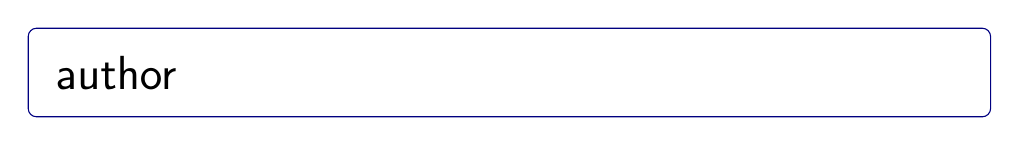
\begin{tikzpicture}
\node[rectangle,rounded corners=3pt,inner sep=10pt,draw=blue!50!black,text width= 0.95\textwidth] {\LARGE \@author};
\end{tikzpicture}
\end{minipage}
\bigskip\bigskip
}%
\makeatother

% custom section
\usepackage[explicit]{titlesec}
\newcommand*\sectionlabel{}
\titleformat{\section}
  {\gdef\sectionlabel{}
   \normalfont\sffamily\Large\bfseries\scshape}
  {\gdef\sectionlabel{\thesection\ }}{0pt}
  {
\noindent
\begin{tikzpicture}
\node[rectangle,rounded corners=3pt,inner sep=4pt,fill=blue!50!black,text width= 0.95\columnwidth] {\color{white}\sectionlabel#1};
\end{tikzpicture}
  }
\titlespacing*{\section}{0pt}{15pt}{10pt}


% custom footer
\usepackage{fancyhdr}
\makeatletter
\pagestyle{fancy}
\fancyhead{}
\fancyfoot[C]{\footnotesize \textcopyright\ \@date\ \ \@author}
\renewcommand{\headrulewidth}{0pt}
\renewcommand{\footrulewidth}{0pt}
\makeatother


\title{Git\ \& \LaTeX\ 101}
\author{Giovanni Grieco, Politecnico di Bari, CC-BY-SA 4.0}
\date{2016}



\begin{document}

\maketitle

\begin{multicols*}{2}


\section{Il lessico di git}

Git è un VCS (\textit{Version Control System}), utile per collaborare con più persone su un progetto.
Chiunque in grado di usare git può salvare (\verb|clone| per lavorare sul progetto principale o \verb|fork| per lavorare indipendentemente) sul proprio computer una copia (\verb|respository|) del codice sorgente (\verb|source|), modificare e salvare (\verb|commit|) i cambiamenti al codice e pubblicare una propria versione (\verb|push|) oppure chiedere che le modifiche siano incluse nel progetto principale (\verb|pull request|). Spesso questo avviene grazie alle segnalazioni (\verb|issues|) da parte degli utenti, che non sanno modificare il codice. I volontari possono discutere liberamente la miglior soluzione possibile e risolvere il problema.

Spesso per tenere in ordine il progetto si possono usare più copie dello stesso (\verb|branch|) come se fossero rami di un albero di sviluppo. Una volta che l'amministratore ritiene opportuno effettuare i cambiamenti sulla copia originale, unirà (\verb|merge|) quelle modifiche effettuate su quel ramo in quello principale (\verb|master branch|). Se il risultato è stabile e soddisfacente, è possibile marcare l'operazione con un'etichetta (\verb|tag|) che servirà per pubblicare la versione compilata al resto dell'utenza (\verb|release|).\footnote{Queste operazioni hanno molto a che fare con l'ingegneria. Spesso nei grandi progetti, come ad esempio i sistemi operativi, esiste una branca dell'ingegneria che si occupa di stabilire se una versione è stabile a tal punto da poter essere pubblicata o meno, denominata \textit{Release Engineering}.}

Git tiene conto delle tue contribuzioni: ogni \verb|commit| è firmato digitalmente dal tuo nome, cognome e indirizzo email. Chiunque quindi potrà accreditare l'autore del cambiamento, sempre se rispettasse la licenza che protegge il progetto e l'autore principale.

\section{GitHub}

GitHub\footnote{Non si devono confondere git e GitHub. Git è un programma installabile ovunque, è libero e open-source. GitHub offre l'infrastruttura con git incluso senza preoccuparsi di nulla se non del proprio codice.} è una piattaforma proprietaria e a fini commerciali che permette di gestire repository git in semplicità. Di norma è possibile utilizzare git via riga di comando o con un programma provvisto di interfaccia grafica, ma la versione web di GitHub è la più semplice e con tante altre funzionalità.

Ogni respository su GitHub ha le seguenti sezioni (si citano solo le principali): \textit{code, issues, pull requests, wiki, releases}.
\begin{itemize}
    \item \textbf{Code}: è possibile sfogliare i file che compongono il progetto, revisionarli e commentarli. È anche possibile visionare la storia delle modifiche cliccando su \textit{commits}.
    \item \textbf{Issues}: permette di segnalare o suggerire un qualcosa, aprendo dibattiti e discussioni tra chiunque partecipi al progetto. I commenti possono essere scritti anche con del testo ben formattato e ricco di contenuti utilizzando il linguaggio \textit{Markdown}. I commit possono essere relazionati alla Issue con un codice che appare affianco al titolo di questa. L'amministratore, quando riterrà opportuno, potrà chiudere la issue.
    \item \textbf{Pull Requests}: chiunque abbia scritto un commit, ma non è amministratore del progetto, può chiedere che le sue modifiche siano revisionate e aggiunte. Questa scheda raccoglie tutte le richieste ed è possibile discuterne fino alla chiusura da parte di un amministratore.
    \item \textbf{Wiki}: serve per scrivere documentazione che riguarda il progetto, magari per semplificare e chiarire il lavoro oppure specificare delle procedure che i volontari devono seguire.
    \item \textbf{Releases}: raccoglie le release e offre al pubblico la possibilità di scaricare sia il progetto compilato che il codice sorgente risalente a quei specifici tag. Questa pagina può essere utile da parte degli utenti per poter scaricare sempre la versione stabile più recente.
\end{itemize}

\section{\LaTeX}
\LaTeX\ permette di scrivere documenti formattati automaticamente, in modo tale che tu possa contentrarti solo sul contenuto. Secondo questa filosofia, LaTeX si propone come un semplice linguaggio costituito per la maggior parte da macro (\textit{comandi}) e pacchetti che aiutano a realizzare il contenuto da scrivere.

Scrivere un documento è molto semplice, basta specificare a LaTeX la tipologia del documento (come libro, o un tema, o un template personalizzato) e scrivere:
\begin{verbatim}
% ho intenzione di scrivere un articolo
% e specifico un font da 12 punti
\documentclass[12pt]{article}
\begin{document}
    Questo è il mio primo documento in LaTeX!
\end{document}
\end{verbatim}

Si può notare che i comandi in LaTeX iniziano con il carattere \textit{backslash} (\verb|\|) e possono avere due tipi di argomenti: quelli mandatori, delimitati da \verb|{...}|, e quelli facoltativi \verb|[...]|. Questi ultimi possono essere, appunto, omessi e LaTeX userà i valori di default specificati nel pacchetto usato (in questo caso la classe \verb|article|). Il carattere percentuale (\%) permette di scrivere commenti sulla riga che saranno ignorati durante la compilazione.

LaTeX è molto usato nella comunità scientifica, quindi non può mancare un motore per gestire e interpretare le equazioni. Le equazioni possono essere introdotte in linea se sono scritte nella forma \verb|$E = mc^{2}$| ($E=mc^2$), oppure su una riga propria e con un carattere più grande \verb|$$E = mc^{2}$$| (\textit{modalità display}): $$E = mc^{2}$$

Infine, creare una testata è semplice e ci sono comandi appositi per formattare per bene la copertina:
\begin{verbatim}
% articolo con font da 12 punti
\documentclass[12pt]{article}
% specifico la codifica (Unicode 8bit)
\usepackage[utf8]{inputenc}

% specifico il titolo
\title{Il mio primo documento}
% specifico autore (con ringraziamenti a piè di pagina)
\author{James T. Kirk \thanks{sponsorizzato da NCC-1701}}
% data di pubblicazione
\date{Novembre 2016}

\begin{document}

% formatto la copertina: 
\begin{titlepage}
\maketitle
\end{titlepage}

Questo è il mio primo documento, e questo è il contenuto
che sto scrivendo.

Una riga vuota permette di scrivere il paragrafo successivo.

Come sempre, un'equazione non fa mai male:
$$f(t) * g(t) \, \stackrel{\mathrm{def}}{=}\ 
\underbrace{\int_{-\infty}^\infty f(\tau)\, g(t - \tau)\, 
d\tau}_{(f * g )(t)}$$
 
\end{document}
\end{verbatim}

Per curiosità riporto qui l'equazione scritta:
$$f(t) * g(t) \, \stackrel{\mathrm{def}}{=}\ \underbrace{\int_{-\infty}^\infty f(\tau)\, g(t - \tau)\, d\tau}_{(f * g )(t)}\footnotemark$$
\footnotetext{Convoluzione di due segnali}

Altre informazioni si possono ritrovare cercando su Google. Per poter iniziare con facilità è possibile usare piattaforme come ShareLaTeX, oppure installare la suite LaTeX sul proprio computer.

\section{Link Utili}
Documentazione di git: \url{https://git-scm.com/doc}\\
Documentazione di GitHub: \url{https://help.github.com}\\
Tutorial interattivo per git: \url{https://try.github.io}\\
Documentazione per LaTeX: \url{https://www.sharelatex.com/learn}\\
StackExchange su LaTeX: \url{http://tex.stackexchange.com}

\section{Su questo documento}
Il codice è reperibile su \href{http://github.com/}{GitHub}. È possibile sperimentare git e poter proporre aggiornamenti per migliorare il documento (oppure semplicemente testare le funzionalità). \verb|Pull Request| di qualsiasi natura sarà accettato in una branch a parte.

\end{multicols*}

\end{document}
